\documentclass[a4paper,12pt]{article}
\usepackage[utf8]{inputenc}
\usepackage{fancyhdr}
\usepackage{graphicx}
\usepackage{lastpage}
\graphicspath{ {./report_images/} }

\pagestyle{fancy}


\lhead{Control \#1924744}
\rhead{Page \thepage \hspace{1pt} of \pageref{LastPage}}

\begin{document}

\title{Insert Title Here}
\author{Control \#1924744}
\date{28th January 2019}
\maketitle
\newpage

\pagenumbering{roman}

\section*{\hfil Summary\hfil}
\begin{center}
\textit{"All models are wrong but some are useful''} \\*
\end{center}

\newpage

\section*{\hfil HELP INC MEMO\hfil}
\newpage


\tableofcontents
\newpage
\pagenumbering{arabic}


\newpage


\section{Introduction}

\subsection{Background}
Puerto Rico is a small US territory situated on the 18th parallel. It has a population of approx 3.29 mill and a population density focused around the coast,
with San Juan being its most popular area$^{1}$. Puerto Rico's tropical climate is starkly divided between the northern two thirds and southern third of the island.
The northern side experiences much more humid weather than the southern side and is the area we are most concerned with.\\* Puerto Rico's annual rainfall also differs greatly between the eastern front, where the Sierra de Luquillo rainforest is located and the western side of the island.
May to November is generally considered to be hurricane season in Puerto Rico while December to March is known as the dry season$^{2}$.
In recent years climate change has caused an acceleration of storms in the tropical belt and poses a serious threat to the future prosperity of Puerto Rico, efforts are ongoing to combat this problem but critics have been outspoken against the lack
of focused effort to deal with it more$^{3}$.
\begin{figure}[h]
\centering
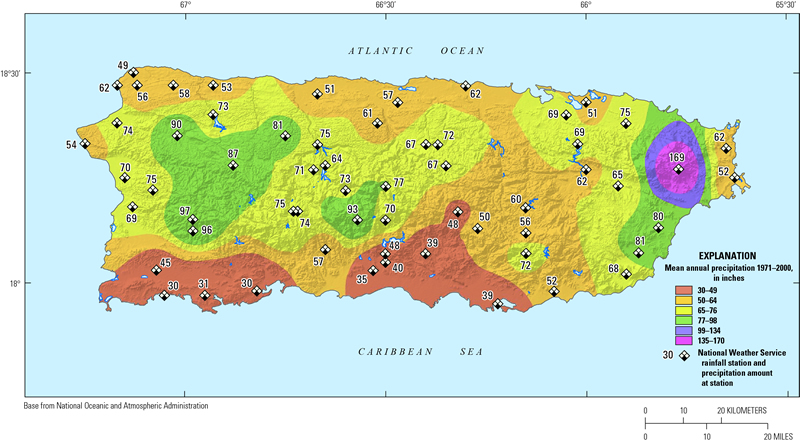
\includegraphics[scale =0.5]{Rainfall}
\caption{Mean Annual Precipitation 1971-2000}
\label{rainfall}
\end{figure}


\subsection{Problem Restatement}
As asked by HELP.INC we were tasked with developing a DroneGo drone fleet that could help deal with future disasters in
Puerto Rico by analyzing the 2017 hurricane. Our task is divided into two main objectives;
\begin{itemize}
\item[-]Delivering required medical packages to the associated medical centres each day.
\item[-]Assessing the major highways and roads that link these centres for ground route planning
\end{itemize}
In order to achieve our first object we decided to start from the bottom and make our way up. That is to say, we began by seeing how to fit medical packages into cargo bay containers, following this
we moved onto seeing which CB-MP (cargo bay to medical package) combination would suit each medical centre's daily needs. Moving up the ladder we ranked our drones by maximum range and so forth and so on.
\\*One major problem appeared to be where to leave a container and how to pack items into a container, we recognized this as an optimization problem to solve, specifically a 'bin packing problem'.

\section{Terminology}
Throughout the paper Acronyms and numbers may be used to abbreviate repeated words and terms. While these are usually explained elsewhere they can also be found here for convenience.

\begin{center}
\begin{tabular}{ |c|l| }
\hline
 Acronym & Explanation  \\\hline
 CB & Cargo Bay Container  \\
 MP or P & Medical Package \\
 MC & Medical Centre\\
 C & Container \\
 \hline
\end{tabular}
\end{center}
The following medical centres were also represented using numbers in the maps found in subsequent sections.

\begin{center}
\begin{tabular}{ |c|l| }
 \hline
 Number & Medical Centre  \\\hline
 1 & Caribbean Medical Centre, Fajardo not accurate  \\
 2 & Hospital HIMA, San Pablo \\
 3 & Hospital Pavia Santurce, San Juan \\
 4 & Puerto Rico Children's Hospital, Bayamon \\
 5 & Hospital Pavia Arecibo, Arecibo  \\
 \hline
\end{tabular}
\end{center}

\section{The Assumptions}
The following core assumptions were made before embarking on our first model. These were necessary to fully understand the strategy we would
need to develop to distribute medical supplies and survey roads:

\begin{itemize}
\item[-]Each drone must return to a container after completing one or more deliveries.
        This is because we assume drones must be recharged/restocked before setting out again.
\item[-]Drones can only be used once a day. Drone LiPo batteries are some of the slowest charging batteries around$^{4}$ and
        the size of the drone suggests recharging will take an entire day.
\item[-]Drones could not be recharged at medical centres.
        Initially we considered charging them in the centres but after research, discovered that
        many hospitals in the 2017 crises were without power or generator fuel.
\item[-]The contents of every container will not be damaged or suffer from any accidental malfunction.
\item[-]Major roads and highways can be approximated as straight lines or a zigzag of lines when needed. This is justified as small road deviations will only be slightly longer than straight lines.
\item[-]Drones are given special permission to fly in airport airspace. This is because otherwise drone delivery in San Juan would be impossible otherwise as the medical centres are in airspace.
\item[-]Containers cannot be left directly in front of hospitals, due to road damage. This assumption was necessary later on.
\item[-]Drones are assumed to be unable to glide. If drones could glide then only one container would be theoretically necessary however this is too unlikely.
\end{itemize}

\section{The Ideal Setup}

\subsection{P-CB (Package to Cargo Bay) Configuration}

In order to understand which drone was suitable to use in deliveries it was necessary to begin with the core fundamentals
of how a cargo bay would store medical packages. This was again noticed to be a bin packing problem however we In order to visualize this a table was generated for the
different combinations of medical packages each cargo bay could carry.\\*
In the table below the different maximum loads each cargo bay can hold is shown.\\*
$m_x =$ medical package $x$


\begin{center}
\begin{tabular}{ |c|l| }
 \hline
 Cargo Bay 1 & ${(m_1),(m_2),(m_3)}$  \\
 Cargo Bay 2 & ${(m_1),(m_2,m_2,m_2),(m_3,m_3),(m_1,m_2)(m_2,m_3)}$  \\
 \hline
\end{tabular}
\end{center}

As seen in the table cargo bay 1 is limited to sending one medical package per drone whereas cargo bay 2 has much
more flexible types of combinations available.
We will next look at the daily needs of each medical center and the associated CB deliveries that would be available.

\subsection{CB combinations for medical centres}
\begin{center}
\begin{tabular}{ |c|c|c|c| }
 \hline
 MC & Daily Need & CB1 & CB2 \\\hline
  1 & $(m_1,m_3)$ & $(m_1),(m_3)$ & $(m_1),(m_2,m_3),(m_3,m_3)$  \\
  2 & $(m_1,m_1,m_3)$ & $(m_1),(m_1),(m_3)$ & $(m_1),(m_1),(m_2,m_3),(m_3,m_3)$  \\
  3 & $(m_1,m_2)$ & $(m_1),(m_2)$ & $ (m_2,m_1)$  \\
  4 & $(m_1,m_1,m_2,m_3,m_3)$ & $(m_1),(m_1),(m_2),(m_3),(m_3)$ & $(m_1),(m_1),(m_2,m_3),(m_3,m_3)$  \\
  5 & $(m_1)$ & $(m_1)$ & $(m_1)$  \\
\hline
\end{tabular}
\end{center}
Looking at the table we can see that 3 and 5 both have available CB's that match their daily needs (CB1 and CB2 respectively).
For the others, it is harder to immediately see which configuration will suit them.\\*
It is now important to determine a strategy by which these CB's will be delivered to each location.

\section{Containers and Locations}
\subsection{Eliminating Unnecessary Drones}
Looking at the requirements of each medical centre it is obvious that the most important factor is the range a drone can travel rather than the speed.
This is because a drone that arrives 40mins earlier is trivial when operating on a 24hr deadline for delivery.
We then proceeded to rank drones in terms of their distance as well as if they were a CB1 or CB2 type drone.
Drones A and H were immediately discarded as they either completely useless for the task required or simply very inefficient.

\begin{center}
\begin{tabular}{ |c|c|c| }
 \hline
 Drone & Distance (Km) & CB \\\hline
  B & 24.4 & 1 \\
  C & 17.1 & 2  \\
  D & 7.9 & 1 \\
  E & 6.5 & 2 \\
  F & 14.4 & 2 \\
  G & 7.5 & 2 \\
 \hline
\end{tabular}
\end{center}
Looking at the table we can see that the best CB1 drone is drone B, likewise the best CB2 drone is drone C. At second place are drones D and F respectively.

\subsection{Drone Flight Radius}
Before developing a configuration for each container it was important to see where containers could be placed regardless of their packing.
Using simple geometry and a generated map of Puerto Rico we could instantly visualize the radial distance a drone could travel from a medical centre.\\*
The region that intercepted each circle would tell us where we could place a container. This allowed us to immediately discard any unsuitable area and focus on where the circle boundaries overlapped.
\\*We also imposed a few local assumptions to realistically reflect each drone's performance.

\begin{itemize}
\item[-]Drones would have a 5 percent range reduction due to carrying a large payload
\item[-]Drones would have a 400 feet (122m) range reduction due to having to climb to (at most) that altitude before travel.
\end{itemize}

\begin{figure}[p]
\centering
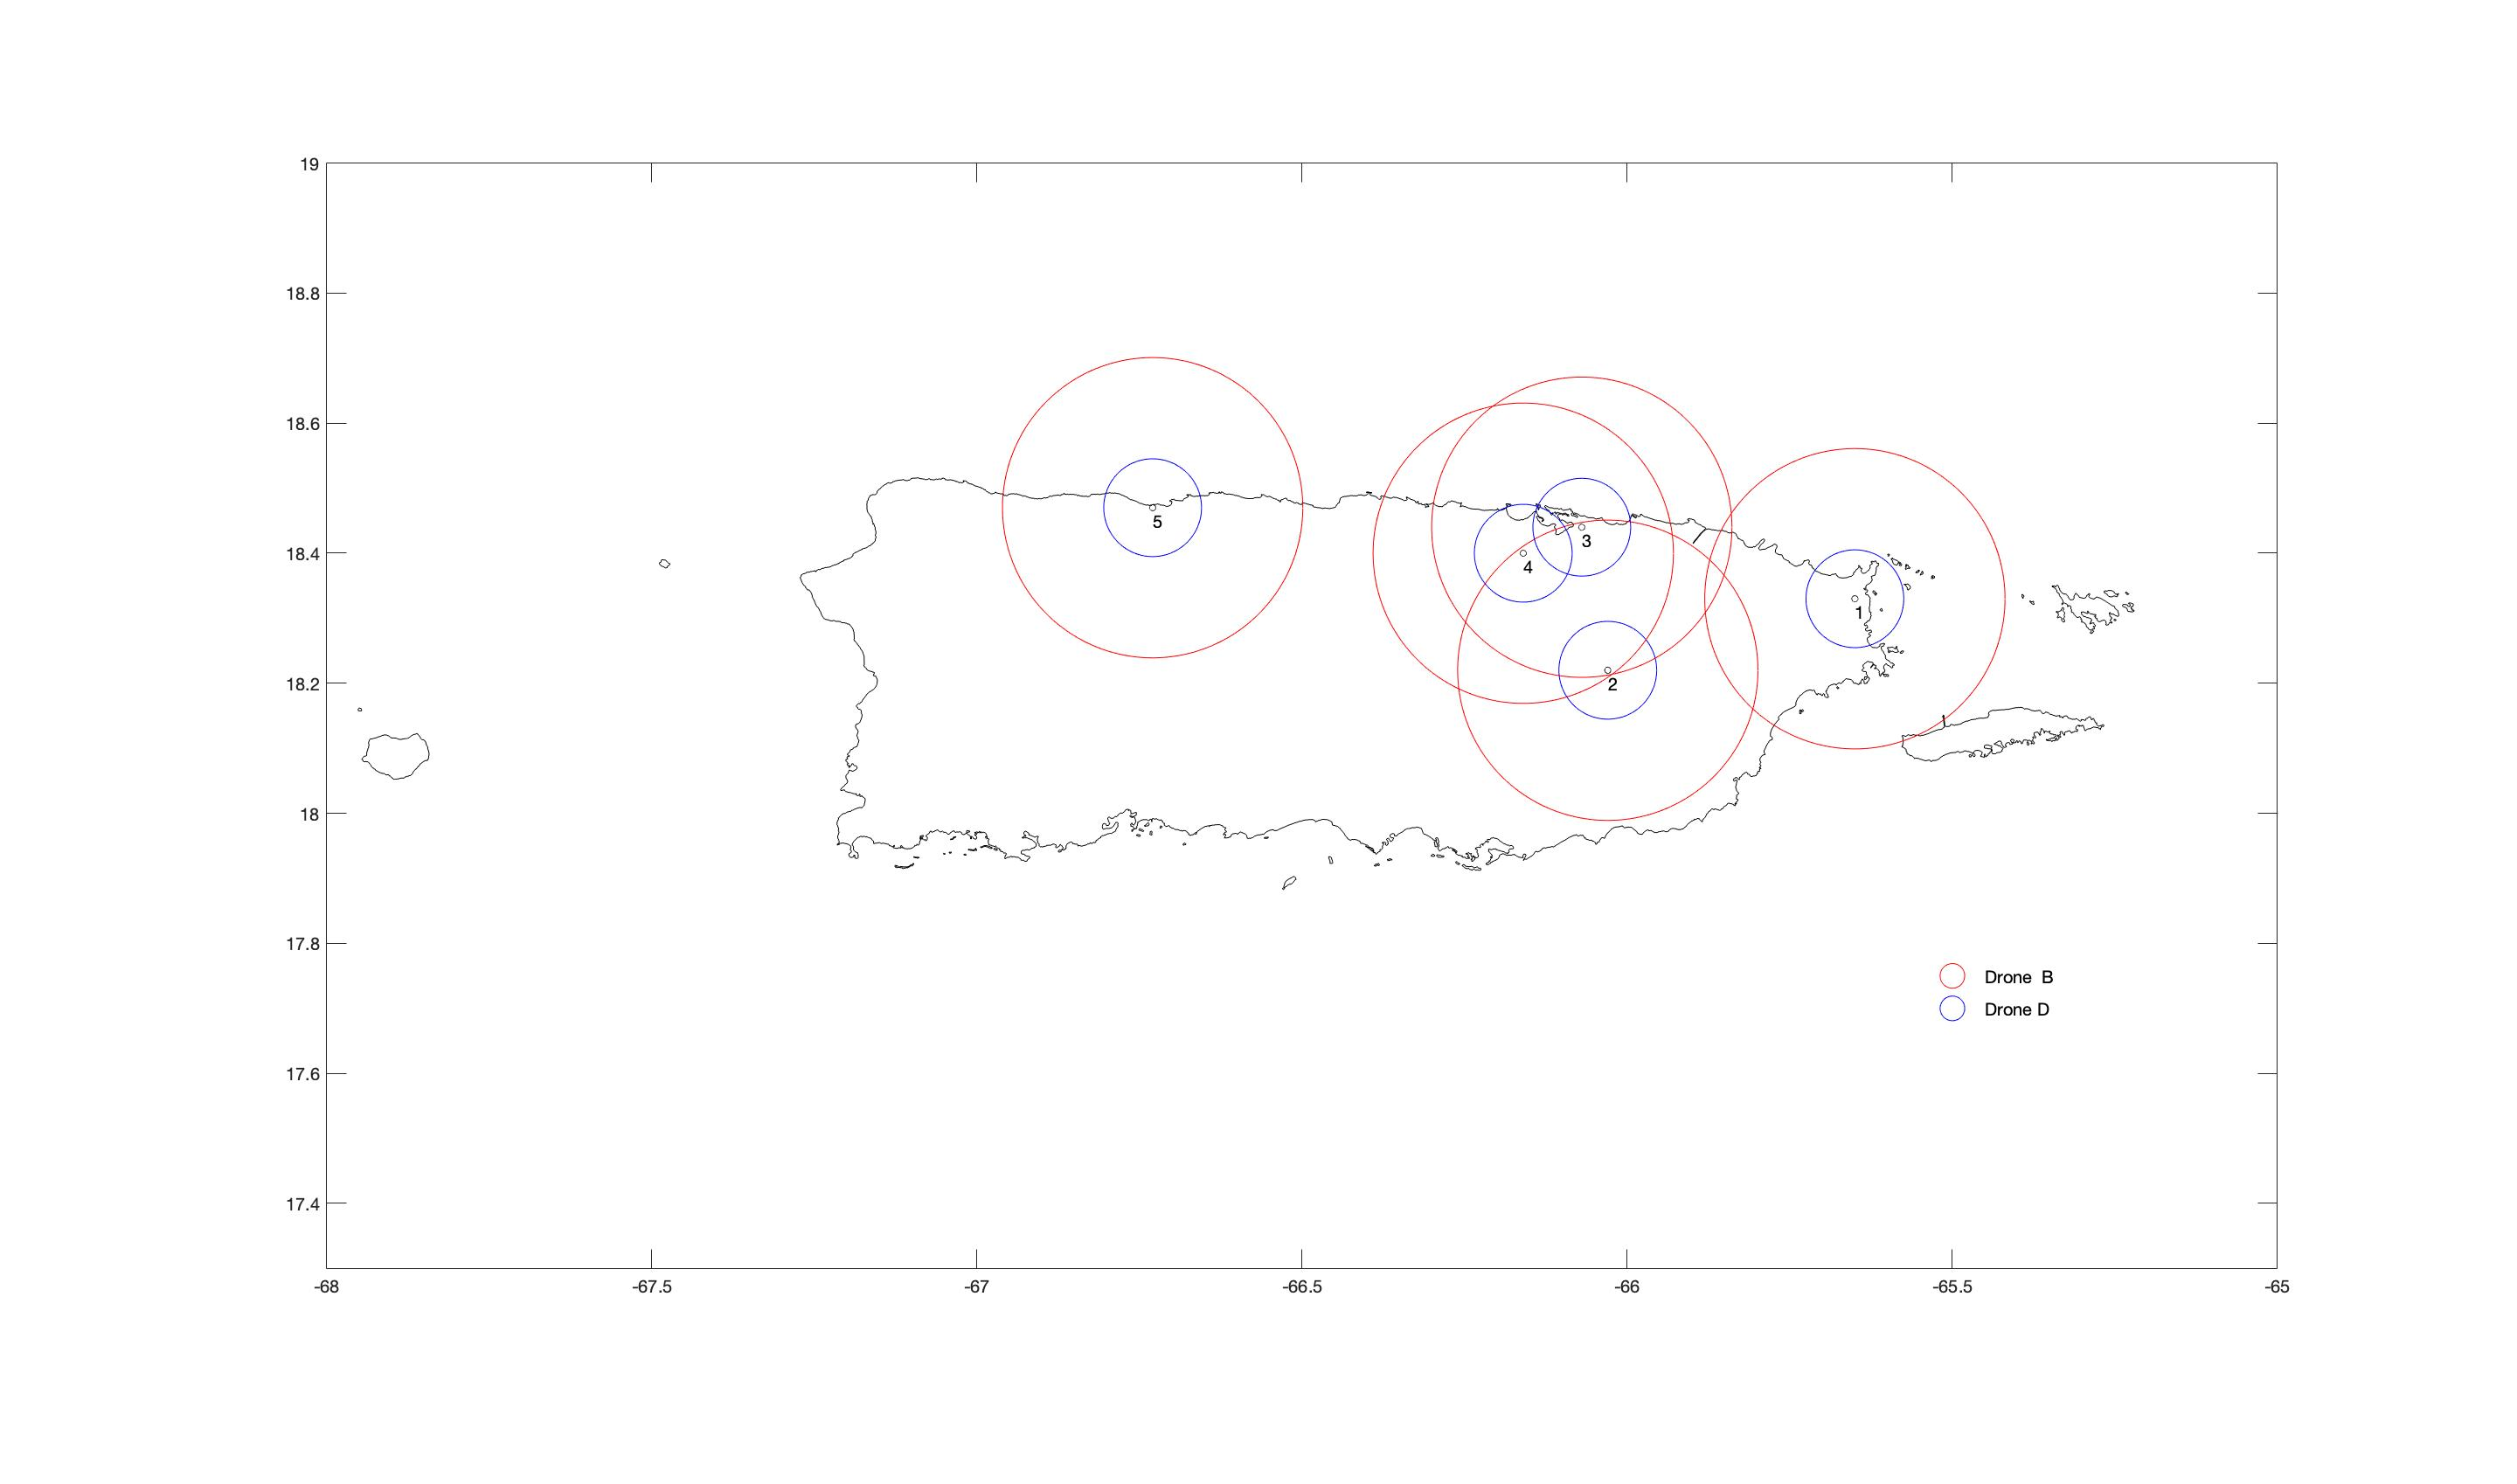
\includegraphics[scale =0.15]{CB1}
\caption{CB1 drone radii around each MC}
\label{cb1}
\end{figure}

\begin{figure}[p]
\centering
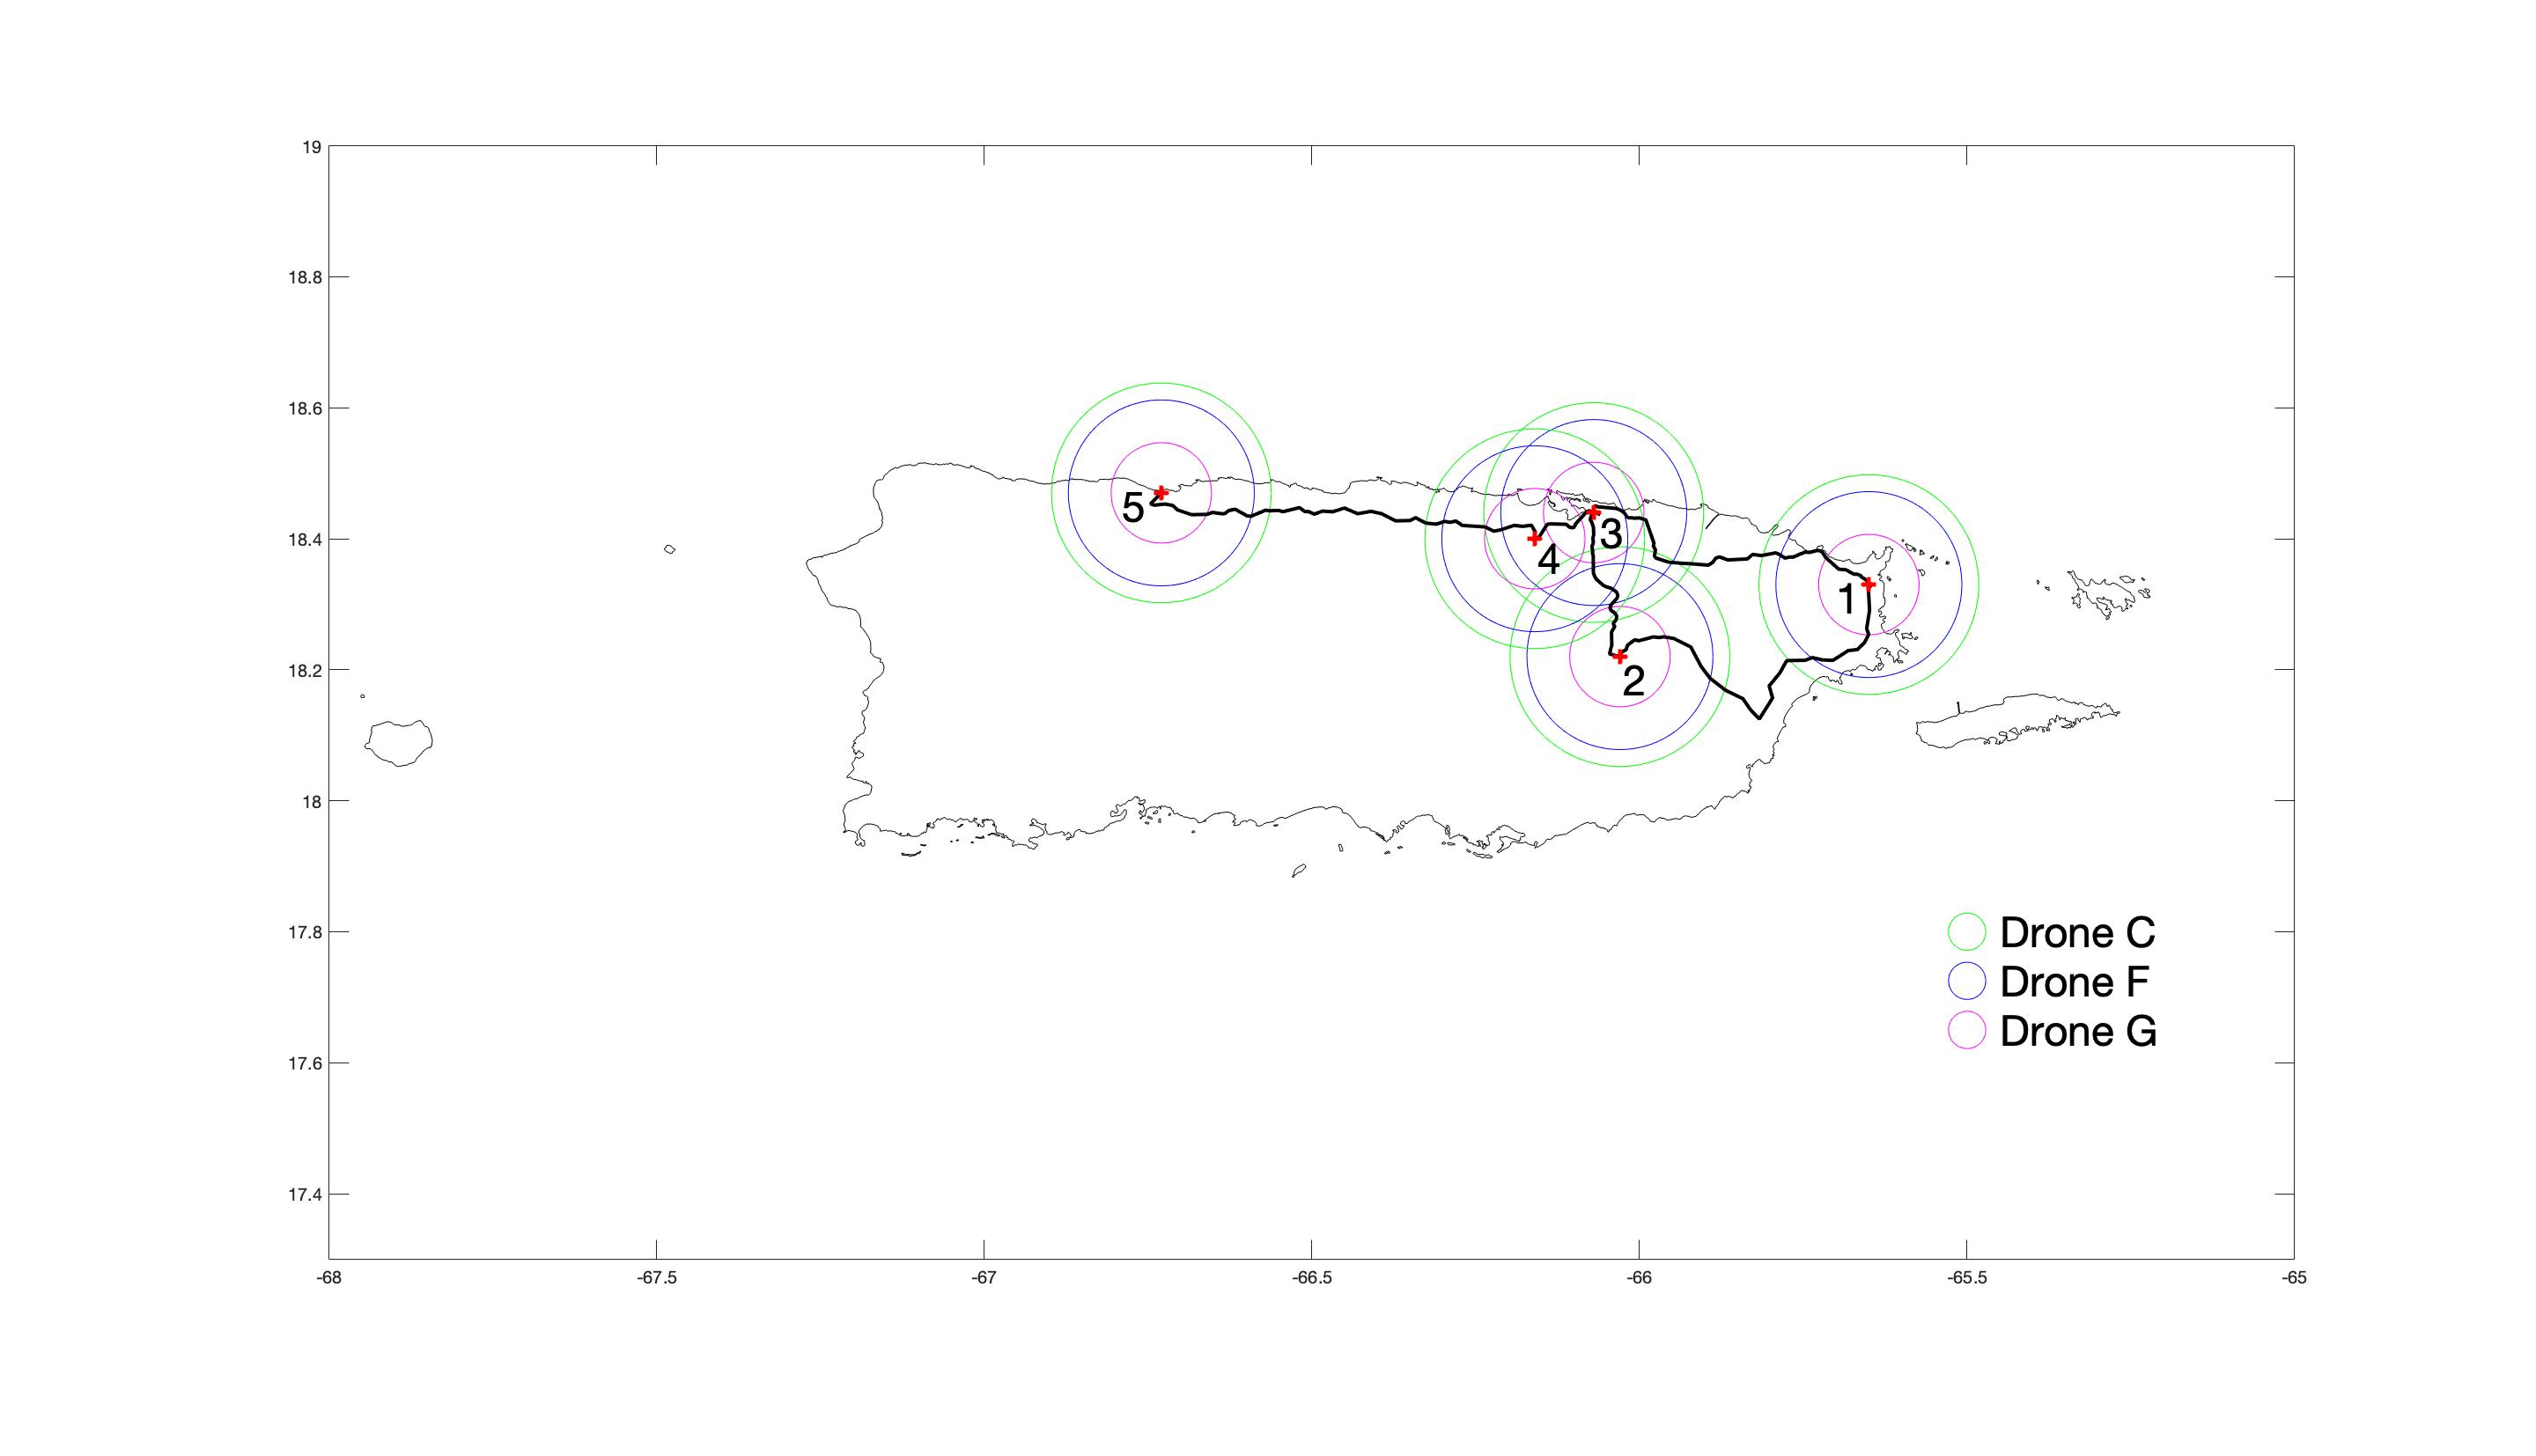
\includegraphics[scale =0.15]{CB2}
\caption{CB2 drone radii around each MC}
\label{cb2}
\end{figure}

\newpage

\subsection{Number of Containers to use}
Ideally a minimum number of containers should be used to appropriately distribute resources in order to minimize costs.
However looking at the diagrams above we can see that MC1 and MC5 are completely separated from any other MC regardless
of which drone we use$^{*}$. This means that \bf{we must require all three containers} \normalfont{to deliver medical packages to each medical centre.
Since we need three containers we will call them C1, C2 and C3 to save time. Each container will serve the following MCs:}

\begin{center}
\begin{tabular}{ |c|c| }
 \hline
 Container & Medical Centres Served \\\hline
  C1 & MC1 \\
  C2 & MC2, MC3, MC4  \\
  C3 & MC5 \\
 \hline
\end{tabular}
\end{center}

We can now look at each individual container and determine the packing configuration we want to serve their respective MCs.
\\**B can technically service MC1, MC2 and MC3 however then it wouldn't service MC4 which makes means its no more effective than the others.
\section{Container Packing Strategy}
In order to solve the problem of packing 3 unique MPs and a drone/s into a container we decided to research bin packing algorithms.
However we were unable to find an algorithm that satisfactorily answered this question.
We therefore resorted to developing our own algorithm which we called the \bf{'Cuboid Reduction Method'} \normalfont{that would be able to
efficiently pack different medical packages into the same container.}
\subsection{Cuboid Reduction Method (CRM)}
Our method known as the cuboid reduction method relies on dividing our container into X amount of cuboids with equal dimensions. We then pack each cuboid with only one
type of medical package to avoid the multi-box fitting scenario (fitting three different boxes into a container). In order to make sure we have the correct balance of each MP we
look at the ratio of the MPs to each other and assign the same ratio of cuboids.\\*
(E.g: A container is split into 10 equally sized cuboids. The associated Medical Centre requires a 1:1 ratio of MP1 and MP2 packages. Thus we assign 5 cuboids for MP1 and 5 cuboids for MP2.

\subsection{Improving the CRM}

\newpage

\section{Mapping Roads}
In order to balance delivering supplies with performing road reconnaissance we first calculated the maximum packing capabilities of C1,C2 and C3.
Since C1 and C3 only serve MC1 and MC5 they can contain a huge amount of supplies. This led us to deciding to allocate an additional Drone to C1 and C3 for pure Recon activities.
This way, one drone will deliver the daily MPs to the MC while another drone scans the different roads in the area.\\*
There are a few caveats to this procedure, firstly, C2 will not have a drone specifically for recon as supplies are too valuable.
Secondly, a drone will travel along approximate straight lines in order to minimize fuel waste. Determining how many straight lines to approximate a road by was done later once the exact coordinates of C1,C2 and C3 were decided.


While C1 and C3 could be dropped anywhere within the red circles of Fig 2, we noticed that since the recon drone is designed to purely assess roads it would be ideal to drop a container on the intersection between the circles circumference and a major road.
This would allow our delivery drone to safely deliver supplies while having the recon drone start immediately on a major highway rather than waste fuel going towards one.
\subsection{Approximating Road Distances}
\subsection{Road Recon Model (RRM)}


\newpage

\section{Performance Evaluation}

\newpage

\section{Sensitivity Analysis}

\newpage

\section{Conclusions}

\newpage

\section{Appendices}
1 - Puerto Rico CIA World Factbook
2 - USGS
3 - <An assessment of the impacts of climate change on Puerto Rico's Cultural Heritage with a case study on sea-level rise, October 2017, https://www.sciencedirect.com/science/article/pii/S1296207417306441>
4- https://rogershobbycenter.com/lipoguide/
5 -
\end{document}
